\documentclass[ignorenonframetext,]{beamer}
\setbeamertemplate{caption}[numbered]
\setbeamertemplate{caption label separator}{: }
\setbeamercolor{caption name}{fg=normal text.fg}
\beamertemplatenavigationsymbolsempty
\usepackage{lmodern}
\usepackage{amssymb,amsmath}
\usepackage{ifxetex,ifluatex}
\usepackage{fixltx2e} % provides \textsubscript
\ifnum 0\ifxetex 1\fi\ifluatex 1\fi=0 % if pdftex
  \usepackage[T1]{fontenc}
  \usepackage[utf8]{inputenc}
\else % if luatex or xelatex
  \ifxetex
    \usepackage{mathspec}
  \else
    \usepackage{fontspec}
  \fi
  \defaultfontfeatures{Ligatures=TeX,Scale=MatchLowercase}
\fi
\usefonttheme{structurebold}
% use upquote if available, for straight quotes in verbatim environments
\IfFileExists{upquote.sty}{\usepackage{upquote}}{}
% use microtype if available
\IfFileExists{microtype.sty}{%
\usepackage{microtype}
\UseMicrotypeSet[protrusion]{basicmath} % disable protrusion for tt fonts
}{}
\newif\ifbibliography
\usepackage{color}
\usepackage{fancyvrb}
\newcommand{\VerbBar}{|}
\newcommand{\VERB}{\Verb[commandchars=\\\{\}]}
\DefineVerbatimEnvironment{Highlighting}{Verbatim}{commandchars=\\\{\}}
% Add ',fontsize=\small' for more characters per line
\usepackage{framed}
\definecolor{shadecolor}{RGB}{248,248,248}
\newenvironment{Shaded}{\begin{snugshade}}{\end{snugshade}}
\newcommand{\KeywordTok}[1]{\textcolor[rgb]{0.13,0.29,0.53}{\textbf{{#1}}}}
\newcommand{\DataTypeTok}[1]{\textcolor[rgb]{0.13,0.29,0.53}{{#1}}}
\newcommand{\DecValTok}[1]{\textcolor[rgb]{0.00,0.00,0.81}{{#1}}}
\newcommand{\BaseNTok}[1]{\textcolor[rgb]{0.00,0.00,0.81}{{#1}}}
\newcommand{\FloatTok}[1]{\textcolor[rgb]{0.00,0.00,0.81}{{#1}}}
\newcommand{\ConstantTok}[1]{\textcolor[rgb]{0.00,0.00,0.00}{{#1}}}
\newcommand{\CharTok}[1]{\textcolor[rgb]{0.31,0.60,0.02}{{#1}}}
\newcommand{\SpecialCharTok}[1]{\textcolor[rgb]{0.00,0.00,0.00}{{#1}}}
\newcommand{\StringTok}[1]{\textcolor[rgb]{0.31,0.60,0.02}{{#1}}}
\newcommand{\VerbatimStringTok}[1]{\textcolor[rgb]{0.31,0.60,0.02}{{#1}}}
\newcommand{\SpecialStringTok}[1]{\textcolor[rgb]{0.31,0.60,0.02}{{#1}}}
\newcommand{\ImportTok}[1]{{#1}}
\newcommand{\CommentTok}[1]{\textcolor[rgb]{0.56,0.35,0.01}{\textit{{#1}}}}
\newcommand{\DocumentationTok}[1]{\textcolor[rgb]{0.56,0.35,0.01}{\textbf{\textit{{#1}}}}}
\newcommand{\AnnotationTok}[1]{\textcolor[rgb]{0.56,0.35,0.01}{\textbf{\textit{{#1}}}}}
\newcommand{\CommentVarTok}[1]{\textcolor[rgb]{0.56,0.35,0.01}{\textbf{\textit{{#1}}}}}
\newcommand{\OtherTok}[1]{\textcolor[rgb]{0.56,0.35,0.01}{{#1}}}
\newcommand{\FunctionTok}[1]{\textcolor[rgb]{0.00,0.00,0.00}{{#1}}}
\newcommand{\VariableTok}[1]{\textcolor[rgb]{0.00,0.00,0.00}{{#1}}}
\newcommand{\ControlFlowTok}[1]{\textcolor[rgb]{0.13,0.29,0.53}{\textbf{{#1}}}}
\newcommand{\OperatorTok}[1]{\textcolor[rgb]{0.81,0.36,0.00}{\textbf{{#1}}}}
\newcommand{\BuiltInTok}[1]{{#1}}
\newcommand{\ExtensionTok}[1]{{#1}}
\newcommand{\PreprocessorTok}[1]{\textcolor[rgb]{0.56,0.35,0.01}{\textit{{#1}}}}
\newcommand{\AttributeTok}[1]{\textcolor[rgb]{0.77,0.63,0.00}{{#1}}}
\newcommand{\RegionMarkerTok}[1]{{#1}}
\newcommand{\InformationTok}[1]{\textcolor[rgb]{0.56,0.35,0.01}{\textbf{\textit{{#1}}}}}
\newcommand{\WarningTok}[1]{\textcolor[rgb]{0.56,0.35,0.01}{\textbf{\textit{{#1}}}}}
\newcommand{\AlertTok}[1]{\textcolor[rgb]{0.94,0.16,0.16}{{#1}}}
\newcommand{\ErrorTok}[1]{\textcolor[rgb]{0.64,0.00,0.00}{\textbf{{#1}}}}
\newcommand{\NormalTok}[1]{{#1}}
\usepackage{graphicx,grffile}
\makeatletter
\def\maxwidth{\ifdim\Gin@nat@width>\linewidth\linewidth\else\Gin@nat@width\fi}
\def\maxheight{\ifdim\Gin@nat@height>\textheight0.8\textheight\else\Gin@nat@height\fi}
\makeatother
% Scale images if necessary, so that they will not overflow the page
% margins by default, and it is still possible to overwrite the defaults
% using explicit options in \includegraphics[width, height, ...]{}
\setkeys{Gin}{width=\maxwidth,height=\maxheight,keepaspectratio}

% Prevent slide breaks in the middle of a paragraph:
\widowpenalties 1 10000
\raggedbottom

\AtBeginPart{
  \let\insertpartnumber\relax
  \let\partname\relax
  \frame{\partpage}
}
\AtBeginSection{
  \ifbibliography
  \else
    \let\insertsectionnumber\relax
    \let\sectionname\relax
    \frame{\sectionpage}
  \fi
}
\AtBeginSubsection{
  \let\insertsubsectionnumber\relax
  \let\subsectionname\relax
  \frame{\subsectionpage}
}

\setlength{\emergencystretch}{3em}  % prevent overfull lines
\providecommand{\tightlist}{%
  \setlength{\itemsep}{0pt}\setlength{\parskip}{0pt}}
\setcounter{secnumdepth}{0}
\definecolor{links}{HTML}{800080}
\hypersetup{colorlinks,linkcolor=,urlcolor=links}

\title{Web Data Collection with R}
\subtitle{Xpath Case Study}
\author{Peter Meißner / 2016-02-29 -- 2016-03-04 / ECPR WSMT}
\date{}

\begin{document}
\frame{\titlepage}

\begin{frame}
\tableofcontents[hideallsubsections]
\end{frame}

\section{Overview}\label{overview}

\begin{frame}{\ldots{} in which we \ldots{}}

\begin{itemize}
\tightlist
\item
  extract \textbf{links} using \textbf{XPath}
\item
  folow them to \textbf{extract links} again
\item
  and build a \textbf{network} of notable political scientists
\end{itemize}

\end{frame}

\begin{frame}{\ldots{} and learn about \ldots{}}

\begin{itemize}
\tightlist
\item
  \textbf{Xpath}
\item
  \textbf{Selector Gadget}
\end{itemize}

\end{frame}

\begin{frame}{\ldots{} while using packages \ldots{}}

\begin{itemize}
\tightlist
\item
  \textbf{rvest} (information extraction from HTML)
\item
  \textbf{stringr} (string manipulation)
\item
  \textbf{d3Network} (network data visualizetion)
\end{itemize}

\end{frame}

\section{Live coding}\label{live-coding}

\begin{frame}[fragile]{a first glance at the page}

\begin{Shaded}
\begin{Highlighting}[]
\KeywordTok{require}\NormalTok{(rvest)}
\KeywordTok{require}\NormalTok{(stringr)}
\end{Highlighting}
\end{Shaded}

\begin{Shaded}
\begin{Highlighting}[]
\NormalTok{url <-}\StringTok{ }
\StringTok{"https://en.wikipedia.org/wiki/List_of_political_scientists"}

\NormalTok{## browseURL(url)}
\end{Highlighting}
\end{Shaded}

\end{frame}

\begin{frame}{a first try at extracting links}

\begin{itemize}
\tightlist
\item
  lets get all the links
\end{itemize}

\end{frame}

\begin{frame}{a first try at extracting links}

\begin{itemize}
\tightlist
\item
  How shall we do it?
\end{itemize}

\end{frame}

\begin{frame}{a first try at extracting links}

\begin{itemize}
\item
  How shall we do it?
\item
  think first
\item
  looking for similarities
\item
  looking for differences
\item
  using every available tool in conjunction
\end{itemize}

\end{frame}

\begin{frame}[fragile]{a first try at extracting links}

\begin{itemize}
\item
  How shall we do it?
\item
  \texttt{\textless{}a\textgreater{}}-nodes
\item
  href should entail \texttt{/wiki/}
\item
  child of \texttt{\textless{}li\textgreater{}}, child of
  \texttt{\textless{}ul\textgreater{}}
\item
  always 1st child
\item
  XPath: \textbf{\texttt{//ul/li/a{[}1{]}}}
\item
  than do further filter by RegEx
\end{itemize}

\end{frame}

\begin{frame}[fragile]{a first try at extracting links}

\begin{Shaded}
\begin{Highlighting}[]
\NormalTok{html   <-}\StringTok{ }\KeywordTok{read_html}\NormalTok{(url)}
\NormalTok{ankers <-}\StringTok{ }\KeywordTok{html_nodes}\NormalTok{(html, }\DataTypeTok{xpath=}\StringTok{"//a"}\NormalTok{)}
\KeywordTok{length}\NormalTok{(ankers)}
\end{Highlighting}
\end{Shaded}

\begin{verbatim}
## [1] 669
\end{verbatim}

\begin{itemize}
\tightlist
\item
  thereafter using RegEx to get rid of those links that did not lead to
  PDF files
\item
  \textbf{we could also use XPath for filtering}
\end{itemize}

\end{frame}

\begin{frame}[fragile]{a first try at extracting links}

\begin{itemize}
\tightlist
\item
  the links a nodes we are looking for
\end{itemize}

\begin{Shaded}
\begin{Highlighting}[]
\NormalTok{ankers[}\DecValTok{100}\NormalTok{:}\DecValTok{102}\NormalTok{]}
\end{Highlighting}
\end{Shaded}

\begin{verbatim}
## {xml_nodeset (3)}
## [1] <a href="/wiki/Alan_Abramowitz" title="Alan Abramowitz">Alan Abramow ...
## [2] <a href="/wiki/David_Adamany" title="David Adamany">David Adamany</a>
## [3] <a href="/wiki/Temple_University" title="Temple University">Temple U ...
\end{verbatim}

\begin{Shaded}
\begin{Highlighting}[]
\KeywordTok{xml_path}\NormalTok{(ankers[}\DecValTok{100}\NormalTok{:}\DecValTok{102}\NormalTok{])}
\end{Highlighting}
\end{Shaded}

\begin{verbatim}
## [1] "/html/body/div[3]/div[3]/div[4]/ul[1]/li[1]/a"   
## [2] "/html/body/div[3]/div[3]/div[4]/ul[1]/li[2]/a[1]"
## [3] "/html/body/div[3]/div[3]/div[4]/ul[1]/li[2]/a[2]"
\end{verbatim}

\end{frame}

\section{Extracting links of notable political
scientists}\label{extracting-links-of-notable-political-scientists}

\begin{frame}[fragile]{get reasonable subset of links}

\begin{Shaded}
\begin{Highlighting}[]
\NormalTok{ankers <-}\StringTok{ }\KeywordTok{html_nodes}\NormalTok{(html, }\DataTypeTok{xpath=}\StringTok{"//ul/li/a[1]"}\NormalTok{)}
\NormalTok{links  <-}\StringTok{ }\KeywordTok{html_attr}\NormalTok{(ankers, }\StringTok{"href"}\NormalTok{)}
\CommentTok{# according to SelectorGagdget should be around}
\KeywordTok{length}\NormalTok{(links) }
\end{Highlighting}
\end{Shaded}

\begin{verbatim}
## [1] 420
\end{verbatim}

\end{frame}

\begin{frame}[fragile]{fine tuning selection of links}

\begin{Shaded}
\begin{Highlighting}[]
\NormalTok{links_iffer <-}\StringTok{ }\CommentTok{# subsetting links by position}
\StringTok{  }\KeywordTok{seq_along}\NormalTok{(links) >=}\StringTok{ }
\StringTok{    }\KeywordTok{seq_along}\NormalTok{(links)[}\KeywordTok{str_detect}\NormalTok{(links, }\StringTok{"Abramowitz"}\NormalTok{)]  &}\StringTok{ }
\StringTok{  }\KeywordTok{seq_along}\NormalTok{(links) <=}
\StringTok{    }\KeywordTok{seq_along}\NormalTok{(links)[}\KeywordTok{str_detect}\NormalTok{(links, }\StringTok{"John_Zaller"}\NormalTok{)] &}\StringTok{ }
\StringTok{  }\KeywordTok{str_detect}\NormalTok{(links, }\StringTok{"/wiki/"}\NormalTok{)}

\NormalTok{links_index <-}\StringTok{ }\KeywordTok{seq_along}\NormalTok{(links)[links_iffer]}
\NormalTok{links <-}\StringTok{ }\NormalTok{links[links_iffer]}

\KeywordTok{length}\NormalTok{(links)}
\end{Highlighting}
\end{Shaded}

\begin{verbatim}
## [1] 294
\end{verbatim}

\end{frame}

\begin{frame}{Further information on notable political scientists}

\end{frame}

\begin{frame}[fragile]{names}

\begin{Shaded}
\begin{Highlighting}[]
\NormalTok{names <-}\StringTok{ }\KeywordTok{html_attr}\NormalTok{(ankers, }\StringTok{"title"}\NormalTok{)[links_index]}
\NormalTok{names <-}\StringTok{ }\KeywordTok{str_replace}\NormalTok{(names, }\StringTok{" }\CharTok{\textbackslash{}\textbackslash{}}\StringTok{(.*}\CharTok{\textbackslash{}\textbackslash{}}\StringTok{)"}\NormalTok{, }\StringTok{""}\NormalTok{)}
\CommentTok{# maybe needed - Windows e.g. depends on your locale: }
\CommentTok{# Sys.getlocale()}
\CommentTok{# stringi::stri_enc_detect(paste(names, collapse = ""))}
\CommentTok{# names <- iconv(names, "utf8", "latin1")}
\end{Highlighting}
\end{Shaded}

\end{frame}

\begin{frame}{other information might come from their personal
wiki-pages}

\begin{itemize}
\tightlist
\item
  \textbf{links to other notable political scientists}
\item
  universities
\item
  place of birth
\item
  key puplications,
\item
  \ldots{}
\end{itemize}

\end{frame}

\begin{frame}[fragile]{Downloading PS pages - preparation}

\begin{Shaded}
\begin{Highlighting}[]
\CommentTok{# loop preparation}
\NormalTok{baseurl <-}\StringTok{ "https://en.wikipedia.org"}
\NormalTok{HTML    <-}\StringTok{ }\KeywordTok{list}\NormalTok{()}
\NormalTok{Fname   <-}\StringTok{ }\KeywordTok{str_c}\NormalTok{(}\StringTok{"downloads/"}\NormalTok{, }\KeywordTok{basename}\NormalTok{(links), }\StringTok{".html"}\NormalTok{)}
\KeywordTok{dir.create}\NormalTok{(}\StringTok{"downloads"}\NormalTok{, }\OtherTok{FALSE}\NormalTok{)}
\NormalTok{URL     <-}\StringTok{ }\KeywordTok{str_c}\NormalTok{(baseurl, links)}
\end{Highlighting}
\end{Shaded}

\end{frame}

\begin{frame}[fragile]{Downloading PS pages - loop}

\begin{Shaded}
\begin{Highlighting}[]
\CommentTok{# loop}
\NormalTok{for ( i in }\KeywordTok{seq_along}\NormalTok{(links) )\{}
  \CommentTok{# url}
  \NormalTok{url <-}\StringTok{ }\NormalTok{URL[i]}
  \CommentTok{# fname}
  \NormalTok{fname <-}\StringTok{ }\NormalTok{Fname[i]}
  \CommentTok{# download}
  \NormalTok{if ( !}\KeywordTok{file.exists}\NormalTok{(fname) )\{}
    \KeywordTok{download.file}\NormalTok{(url, fname)}
    \KeywordTok{Sys.sleep}\NormalTok{(}\FloatTok{0.8}\NormalTok{)}
  \NormalTok{\} }
  \CommentTok{# read in files}
  \NormalTok{HTML[[i]] <-}\StringTok{ }\KeywordTok{read_html}\NormalTok{(fname)}
\NormalTok{\}}
\end{Highlighting}
\end{Shaded}

\end{frame}

\begin{frame}[fragile]{Gathering data on links to other notable PS}

\begin{Shaded}
\begin{Highlighting}[]
\CommentTok{# loop preparation}
\NormalTok{connections <-}\StringTok{ }\KeywordTok{data.frame}\NormalTok{(}\DataTypeTok{from=}\OtherTok{NULL}\NormalTok{, }\DataTypeTok{to=}\OtherTok{NULL}\NormalTok{)}

\CommentTok{# loop}
\NormalTok{for ( i in }\KeywordTok{seq_along}\NormalTok{(HTML))  \{}
  \NormalTok{pslinks          <-}\StringTok{ }\KeywordTok{html_attr}\NormalTok{(}
                        \KeywordTok{html_nodes}\NormalTok{(HTML[[i]], }\DataTypeTok{xpath=}\StringTok{"//a"}\NormalTok{), }
                      \StringTok{"href"}\NormalTok{)}
  \NormalTok{links_in_pslinks <-}\StringTok{ }\KeywordTok{seq_along}\NormalTok{(links)[links %in%}\StringTok{ }\NormalTok{pslinks]}
  \NormalTok{links_in_pslinks <-}\StringTok{ }\NormalTok{links_in_pslinks[links_in_pslinks!=i]}
  \NormalTok{connections      <-}\StringTok{ }\KeywordTok{rbind}\NormalTok{(}
                \NormalTok{connections, }
                \KeywordTok{data.frame}\NormalTok{(}
                  \DataTypeTok{from=}\KeywordTok{rep}\NormalTok{(i, }\KeywordTok{length}\NormalTok{(links_in_pslinks)), }
                  \DataTypeTok{to=}\NormalTok{links_in_pslinks}
                  \NormalTok{) }
                      \NormalTok{)  }
\NormalTok{\}}
\end{Highlighting}
\end{Shaded}

\end{frame}

\begin{frame}[fragile]{Gathering data on links to other notable PS}

\begin{Shaded}
\begin{Highlighting}[]
\CommentTok{# results}
\KeywordTok{names}\NormalTok{(connections) <-}\StringTok{ }
\StringTok{  }\KeywordTok{c}\NormalTok{(}\StringTok{"from"}\NormalTok{, }\StringTok{"to"}\NormalTok{)}
\KeywordTok{head}\NormalTok{(connections)}
\end{Highlighting}
\end{Shaded}

\begin{verbatim}
##   from  to
## 1    5  46
## 2    5 154
## 3    5 274
## 4    8  45
## 5    8 123
## 6   10 253
\end{verbatim}

\end{frame}

\begin{frame}[fragile]{Gathering data on links to other notable PS}

\begin{Shaded}
\begin{Highlighting}[]
\CommentTok{# make symmetrical }
\NormalTok{connections <-}\StringTok{ }
\StringTok{  }\KeywordTok{rbind}\NormalTok{(}
    \NormalTok{connections, }
    \KeywordTok{data.frame}\NormalTok{(}
      \DataTypeTok{from=}\NormalTok{connections$to,}
      \DataTypeTok{to=}\NormalTok{connections$from}
    \NormalTok{)}
 \NormalTok{)}
\end{Highlighting}
\end{Shaded}

\end{frame}

\begin{frame}[fragile]{Plot connections}

\begin{Shaded}
\begin{Highlighting}[]
\KeywordTok{require}\NormalTok{(d3Network)}
\end{Highlighting}
\end{Shaded}

\begin{verbatim}
## Loading required package: d3Network
\end{verbatim}

\begin{Shaded}
\begin{Highlighting}[]
\KeywordTok{d3SimpleNetwork}\NormalTok{( connections, }
                 \DataTypeTok{width =} \DecValTok{1000}\NormalTok{, }
                 \DataTypeTok{height =} \DecValTok{900}\NormalTok{, }
                 \DataTypeTok{file=}\StringTok{"connections.html"}\NormalTok{)}
\CommentTok{# browseURL("connections.html")}
\end{Highlighting}
\end{Shaded}

\end{frame}

\begin{frame}{Plot connections}

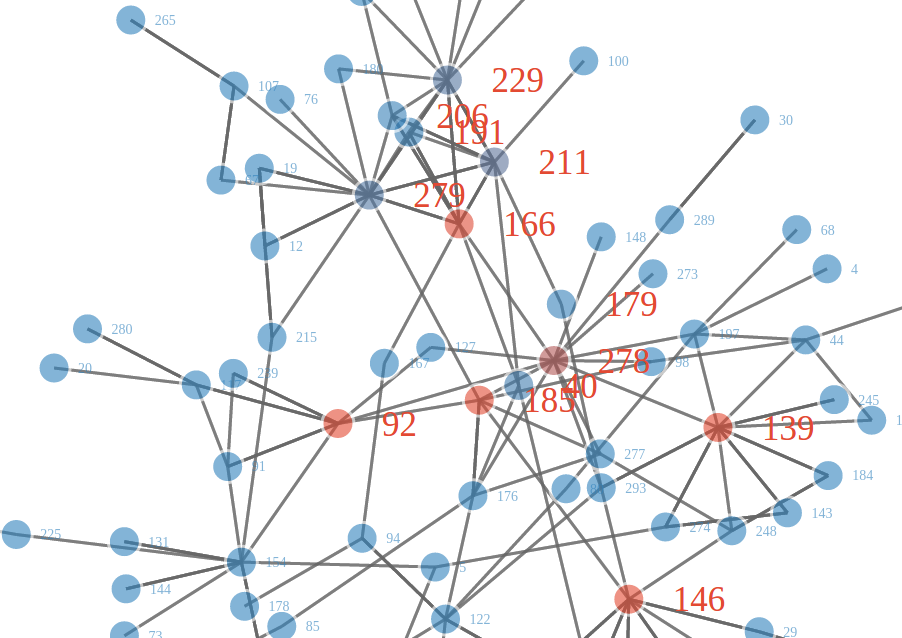
\includegraphics{fig/network1.png}

\end{frame}

\begin{frame}[fragile]{Plot connections}

\begin{Shaded}
\begin{Highlighting}[]
\KeywordTok{d3ForceNetwork}\NormalTok{(}\DataTypeTok{Links =} \NormalTok{connections, }\DataTypeTok{Nodes =} \KeywordTok{data.frame}\NormalTok{(}\DataTypeTok{name =} \NormalTok{names), }\DataTypeTok{Source =} \StringTok{"from"}\NormalTok{, }
    \DataTypeTok{Target =} \StringTok{"to"}\NormalTok{, }\DataTypeTok{opacity =} \FloatTok{0.9}\NormalTok{, }\DataTypeTok{zoom =} \NormalTok{T, }\DataTypeTok{width =} \DecValTok{1000}\NormalTok{, }\DataTypeTok{height =} \DecValTok{900}\NormalTok{, }\DataTypeTok{file =} \StringTok{"connections2.html"}\NormalTok{)}
\CommentTok{# browseURL('connections2.html')}
\end{Highlighting}
\end{Shaded}

\end{frame}

\begin{frame}{Plot connections}

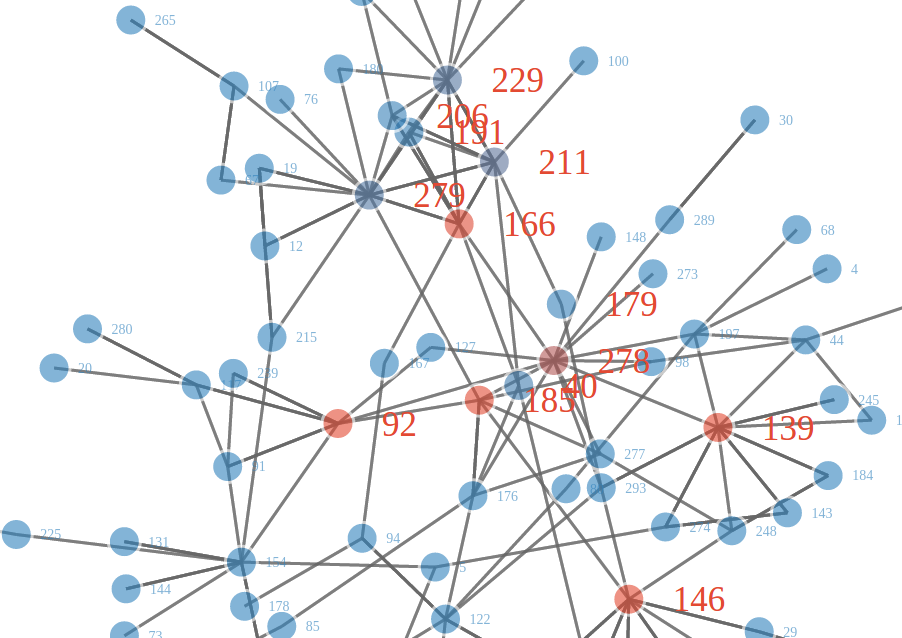
\includegraphics{fig/network1.png}

\end{frame}

\begin{frame}{Plot connections}

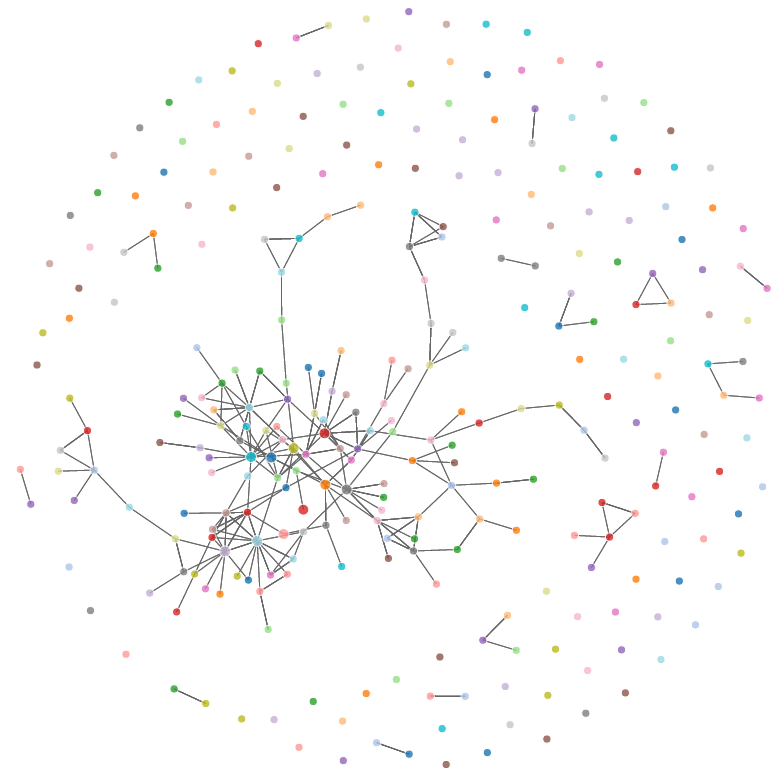
\includegraphics{fig/network2.png}

\end{frame}

\begin{frame}{Plot connections}

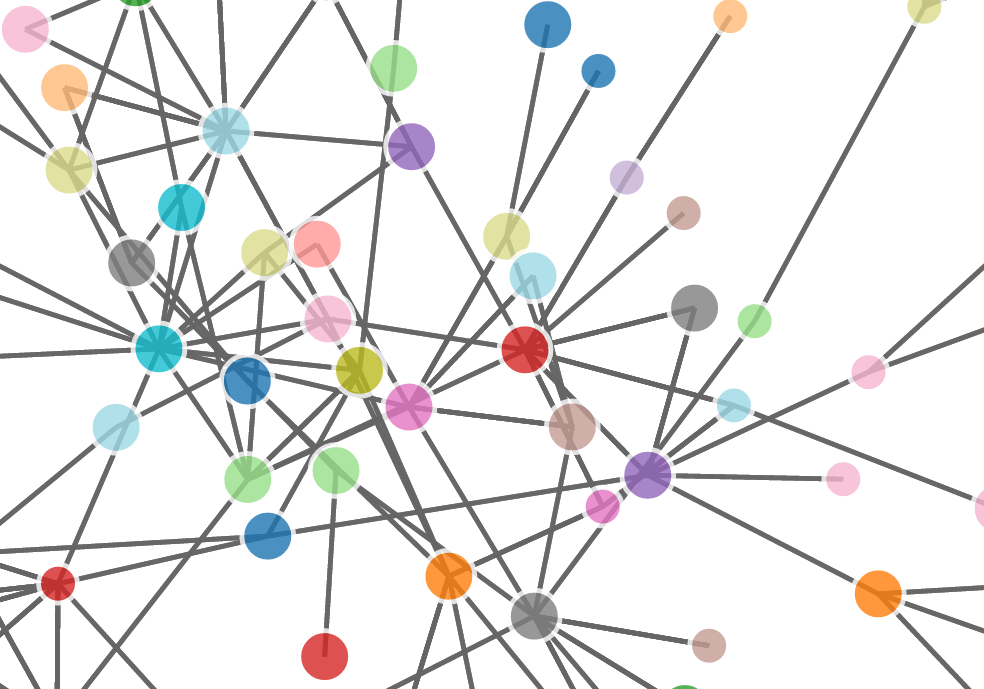
\includegraphics{fig/network3.png}

\end{frame}

\section{Extension}\label{extension}

\begin{frame}{localize notable political scientists}

\begin{itemize}
\tightlist
\item
  go through all PS pages and extract university mentions

  \begin{itemize}
  \tightlist
  \item
    links
  \item
    \ldots{} that have \emph{University}, \emph{School}, \emph{???} in
    text
  \end{itemize}
\item
  think about how to best store/organize this information
\item
  go get it
\item
  geocode universities similar to scenario 1
\end{itemize}

\end{frame}

\begin{frame}{localize notable political scientists}

\begin{itemize}
\tightlist
\item
  Wikipedia pages sometimes entail geographic information
\item
  go through all PS pages and extract all links

  \begin{itemize}
  \tightlist
  \item
    keep those links that lead to Wikipedia pages
  \end{itemize}
\item
  go through all page links left and look for geolocations connected to
  the notable political scientist
\end{itemize}

\end{frame}

\begin{frame}{plot all locations gathered on a map}

\begin{itemize}
\tightlist
\item
  have a look at RegEx-Case-Study for ideas on how to do it
\end{itemize}

\end{frame}

\end{document}
